\section{氧化还原反应与电化学}  
\subsection{氧化还原反应的基本概念}

现在我们进一步推广热力学的部分，即引入非体积功。最简单的是电功，而这样的反应为氧化还原反应。

\begin{definition}[氧化还原反应]
氧化还原反应是涉及电子转移或电子对偏向的化学反应。
\end{definition}

我们这里着重区分氧化数（氧化态）和化合价的概念：
\begin{definition}[氧化数和化合价]
  \begin{enumerate}
    \item 氧化态（$ON$）是指化合物中，假设所有共价键均为离子键（电子归属于电负性更大的原子）时某原子的带电量。
    \item 化合价是指化合物中，某原子成键数量，显然非负。
  \end{enumerate}
\end{definition}

依照这个定义，氧化还原反应可以被定义为氧化态发生变化的反应。

我们往往考察这样的一个反应：$$Red_1 + Ox_2  \to Ox_1 + Red_2$$其中$Ox$和$Red$分别是某物质氧化态和还原态的缩写（我们用角标1，2区分两个物质）。但这相对复杂，我们将其分割：

\begin{definition}[电极半反应]
任何氧化还原反应均可拆分为两个半反应：氧化半反应（失去电子，氧化态升高）和还原半反应（得到电子，氧化态降低）。其一般形式为：
$$Red_1- ze^- \to Ox_1 , \quad Ox_2 + ze^- \to Red_2$$
显然氧化过程失去的电子数等于还原过程得到的电子数（电子守恒）。
\end{definition}

下表给出了相关术语:

\begin{definition}[氧化还原反应相关术语]
\begin{center}
\begin{tabular}{c c c c c}
    \toprule
    反应物氧化数 & 电极半反应 & 反应物 & 行为 & 变化为 \\
    \midrule
    升 & 氧化半反应 & 还原剂 \(Red\) & 被氧化 & 氧化产物 \(OP/Ox'\) \\
    降 & 还原半反应 & 氧化剂 \(Ox\) & 被还原 & 还原产物 \(RP/Red'\) \\
    \bottomrule
\end{tabular}
\end{center}
\end{definition}

\subsection{电极电势}

热力学量是宏观的，而单个化学反应的电子转移是微观的，需要建立联系。

\begin{definition}[Faraday（法拉第）常数]
Faraday常数（$F$）是每摩尔电子所携带的电荷量， $F = N_A e$，其数值约为 $F = 96500\ \mathrm{C\cdot mol^{-1}}$。
\end{definition}

Faraday以实验总结了如下规律，其为电化学的基础：

\begin{proposition}[Faraday电解定律（第一、第二定律）]
\begin{enumerate}
    \item 第一定律：电解过程中，电极上沉积或溶解的物质的量（$n$）与通过电解质溶液的电荷量（$Q$）成正比：$n = {Q}/{zF}$，其中 $z$ 为每个离子转移的电子数。
    \item 第二定律：相同电荷量下，不同物质在电极上沉积的质量与其摩尔质量（$M$）除以转移电子数（$z$）成正比：$\frac{m_1}{m_2} = \frac{M_1/z_1}{M_2/z_2}$。
\end{enumerate}
\end{proposition}

对于电学量的讨论必然涉及电势$\phi $及电势差，我们从一个有趣的事实开始：当金属M制作的电极插入含有金属离子$M^{z+}$的盐溶液中，可能发生金属离子吸附、沉积到电极上，或者电极溶解。在这个过程中，由于电荷的累积，电极与溶液产生了电势差：

\begin{definition}[Trasatti绝对电极电势及其推广]
绝对电极电势是金属电极与盐溶液之间因电极-溶液界面电荷积累产生的电势差。即：
$$\varphi_{abs}(M^{z+}/M)=\phi_M - \phi_{sol}, \quad \varphi_{abs}(Ox/Red) = \phi_{Red} - \phi_{Ox} $$
\end{definition}

然而，这些电势是难测的（注意不是不可测），所以我们定义一个基准：

\begin{definition}[标准氢电极与相对电极电势]
标准氢电极（$SHE$）作为参比电极，其标准电极电势在298.15 K下定义为 $\varphi^\circ(H^+/H_2) = 0\ \mathrm{V}$（100 kPa $H_2$，$1\ \mathrm{mol\cdot L^{-1}}\ H^+$）,其绝对量为：

$$\varphi_{abs}(SHE) = (\varDelta_{hyd}G_m^\circ + IE_1^\circ +\frac{1}{2}BDE)/F + \varphi_{correction} = 4.44\text{V}$$

相对电极电势（$\varphi$）是指被测电极与标准氢电极在指定条件下的电势差。标准电极电势（$\varphi^\circ$）是指标准状态下（纯固/液态、$1\ \mathrm{mol\cdot L^{-1}}$ 溶质、100 kPa气体）的电极电势。
\end{definition}

对于一个两电极的电池，其电动势用花体字母$\mathcal{E}$表示：

\begin{proposition}[电动势]
$$\mathcal{E} = \phi_+ -\phi_- =\varphi_{Ox} - \varphi_{Red}  $$
\end{proposition}

我们回忆第一章的热力学条件，当涉及非体积功时，我们给出了热力学的允许条件，结合电功的定义：$$\Delta G < W_f = q U $$假定Gibbs自由能完全做电功：

\begin{proposition}[电极电势与Gibbs自由能的关系]
电极反应的摩尔吉布斯自由能变与电极电势的关系为：
$$\Delta_r G_m = -zF\mathcal{E} =- z F (\varphi_{Ox} - \varphi_{Red})$$

所以其自发要求氧化半反应电极电势大于还原半反应，也就是说：
\begin{enumerate}
  \item 氧化剂电极电势越大，氧化能力越强；
  \item 还原剂电极电势越小，还原能力越强。
\end{enumerate}
\end{proposition}

电极电势往往应用于元素化学，所以我们很自然地考虑某一个元素，有：

\begin{definition}[Latimer（拉蒂默）标准电极电势图]
Latimer图展示了某元素在特定介质（酸性/碱性）中不同氧化态的标准电极电势，按氧化态从高到低（从左到右）排列。每一个箭头上都标注了箭头两端物质之间的电极电势。

结合我们之前的结论，若某物质右侧半反应的电极电势比左侧更正，则该物种容易发生歧化。
\end{definition}
\begin{example}[氮的Latimer标准电极电势图]
  $$
(pH = 0)\quad\text{NO}_3^- \xrightarrow{0.94\ \text{V}} 
\text{HNO}_2 \xrightarrow{1.00\ \text{V}} 
\text{NO} \xrightarrow{1.59\ \text{V}} 
\text{N}_2\text{O} \xrightarrow{1.77\ \text{V}} 
\text{N}_2 \xrightarrow{-0.23\ \text{V}} 
\text{NH}_4^+
$$


$$
(pH =14)\quad\text{NO}_3^- \xrightarrow{0.01\ \text{V}} 
\text{NO}_2^- \xrightarrow{0.46\ \text{V}} 
\text{NO} \xrightarrow{0.76\ \text{V}} 
\text{N}_2\text{O} \xrightarrow{0.94\ \text{V}} 
\text{N}_2 \xrightarrow{-0.73\ \text{V}} 
\text{NH}_3
$$

\end{example}

Latimer标准电极电势图仅仅提供的相邻氧化态物质之间的电极电势。跨越多个氧化态时，需要注意电极电势不是状态函数，以此不具备加和性：

\begin{proposition}[电极电势的计算]
电极电势不能直接相加，但Gibbs自由能变具有加和性。对于一系列氧化态变化：$$\text{OS}_1 \stackrel{z_1, \varphi_1}{\rightarrow} \text{OS}_2 \stackrel{z_2, \varphi_2}{\rightarrow} \text{OS}_3$$则$\text{OS}_3/\text{OS}_1$的电极电势为：
$$\varphi(\text{OS}_3/\text{OS}_1) = \frac{z_1\varphi_1 + z_2\varphi_2}{z_1 + z_2}$$
其中 $z_1$ 和 $z_2$ 为各步转移的电子数，$\varphi_1$、$\varphi_2$ 为对应的电极电势。
\end{proposition}

Frost（弗罗斯特）-Ebsworth（埃布斯沃思）图，即$z\varphi ^\circ-ON$图（与偏摩尔Gibbs自由能-氧化态图等价）更加直观地展示了这个结果（其中$z$指相对于单质转移的电子数）。类似于Jensen（琴生）不等式，我们只需要将需要的三个物质相连，观察形成的折线。如果是上凸的，则意味着中间的物质易发生歧化；如果是下凹的，则意味着两侧的物质易发生归中。

\begin{example}[氮的Frost-Ebsworth图]
  
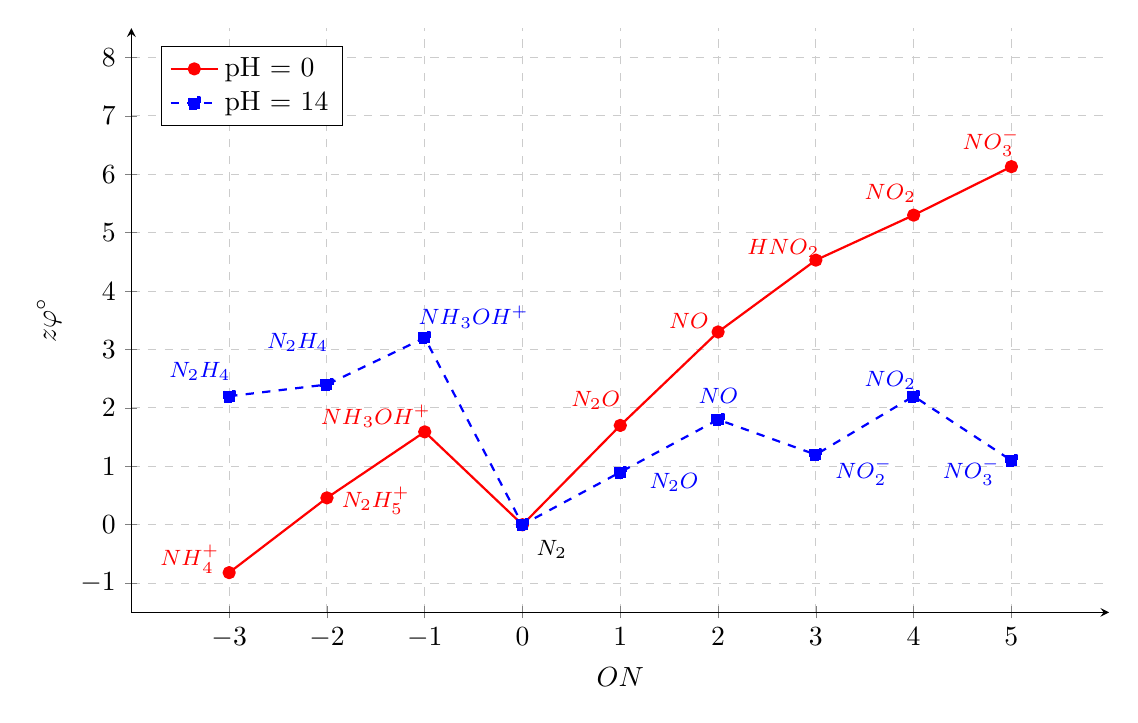
\begin{tikzpicture}
\begin{axis}[
    width=14cm,
    height=9cm,
    xlabel={$ON$},
    ylabel={$z\varphi ^\circ$},
    xmin=-4, xmax=6,
    ymin=-1.5, ymax=8.5,
    xtick={-3,-2,-1,0,1,2,3,4,5},
    ytick={-1,0,1,2,3,4,5,6,7,8},
    grid=major,
    grid style={dashed, gray!40},
    legend pos=north west,
    legend cell align={left},
    axis lines=left,
    enlargelimits=false,
    clip=false,
    every node near coord/.append style={font=\small, anchor=south west},
]



\addplot[
    color=red,
    mark=*,
    thick,
    sharp plot, 
    line join=round
] coordinates {
    (-3, -0.82)  
    (-2, 0.46)  
    (-1, 1.59) 
    (0, 0.00)  
    (1, 1.70) 
    (2, 3.3)
    (3, 4.53)
    (4, 5.3)
    (5, 6.13) 
};
\addlegendentry{pH = 0}

\node[anchor=south east, red, font=\footnotesize] at (axis cs:-3,-1) {$\text{NH}_4^+$};
\node[anchor=south, red, font=\footnotesize] at (axis cs:-1.5,0) {$\text{N}_2\text{H}_5^+$};
\node[anchor=south, red, font=\footnotesize] at (axis cs:-1.5,1.5) {$\text{NH}_3\text{OH}^+$};
\node[anchor=north, black, font=\footnotesize] at (axis cs:0.3,-0.1) {$\text{N}_2$};
\node[anchor=south west, red, font=\footnotesize] at (axis cs:0.4,1.8) {$\text{N}_2\text{O}$};
\node[anchor=south west, red, font=\footnotesize] at (axis cs:1.4,3.2) {$\text{NO}$};
\node[anchor=south west, red, font=\footnotesize] at (axis cs:2.2,4.4) {$\text{HNO}_2$};
\node[anchor=north west, red, font=\footnotesize] at (axis cs:3.4,6) {$\text{NO}_2$};
\node[anchor=south west, red, font=\footnotesize] at (axis cs:4.4,6.13) {$\text{NO}_3^-$};

\addplot[
    color=blue,
    mark=square*,
    thick,
    sharp plot, 
    dashed,
    line join=round
] coordinates {
    (-3, 2.2) 
    (-2, 2.4)  
    (-1, 3.2)  
    (0, 0.00)  
    (1, 0.9)   
    (2, 1.8)  
    (3, 1.2)  
    (4, 2.2) 
    (5, 1.1)    
};
\addlegendentry{pH = 14}
\node[anchor=south, blue, font=\footnotesize] at (axis cs:-3.3,2.3) {$\text{N}_2\text{H}_4$};
\node[anchor=south, blue, font=\footnotesize] at (axis cs:-2.3,2.8) {$\text{N}_2\text{H}_4$};
\node[anchor=south, blue, font=\footnotesize] at (axis cs:-0.5,3.2) {$\text{NH}_3\text{OH}^+$};
\node[anchor=south west, blue, font=\footnotesize] at (axis cs:1.2,0.4) {$\text{N}_2\text{O}$};
\node[anchor=south west, blue, font=\footnotesize] at (axis cs:1.7,1.9) {$\text{NO}$};
\node[anchor=south west, blue, font=\footnotesize] at (axis cs:3.1,0.5) {$\text{NO}_2^-$};
\node[anchor=north west, blue, font=\footnotesize] at (axis cs:3.4,2.8) {$\text{NO}_2$};
\node[anchor=south west, blue, font=\footnotesize] at (axis cs:4.2,0.5) {$\text{NO}_3^-$};

\end{axis}
\end{tikzpicture}

例如，通过连线可以发现：
\begin{enumerate}
  \item 碱性条件下一氧化氮与二氧化氮容易归中，而酸性条件下亚硝酸容易歧化。
  \item 无论是酸性还是碱性，羟胺都容易与亚硝酸（根）归中为氮。
\end{enumerate}

但是如同我们在第一章强调的那样，这是热力学上的允许，而不一定真的发生。

\end{example}

\subsection{条件对电极电势的影响}

我们已经给出了电极电势和Gibbs自由能的关系，结合van't Hoff等温等压方程，给出：

\begin{proposition}[Nernst（能斯特）方程]
$$\varphi = \varphi^\circ - \frac{RT}{zF}\ln\frac{[\text{Red}]}{[\text{Ox}]}$$
298.15 K时，方程简化为：
$$\varphi = \varphi^\circ - \frac{0.0592}{z}\lg\frac{[\text{Red}]}{[\text{Ox}]}$$

所以，最直观地，浓度影响着电极电势：
\begin{enumerate}
    \item 增大 $[\text{Ox}]$、减少$[\text{Red}]$  使 $\varphi$ 升高（氧化性增强）；
    \item 增大 $[\text{Red}]$、减少$[\text{Ox}]$  使 $\varphi$ 降低（还原性增强）。
\end{enumerate}
而且，这种影响对转移电子数更少的反应、在更高的温度更加显著。
\end{proposition}

同样的，沉淀与络合间接地影响着浓度：

\begin{proposition}[沉淀和络合的影响]
\begin{enumerate}
    \item 沉淀：氧化态/还原态形成沉淀会降低其有效浓度，导致氧化态的 $\varphi$ 降低（或还原态的 $\varphi$ 升高）。
    \item 络合：氧化态/还原态形成稳定络合物会降低其有效浓度，效果与沉淀相同。
\end{enumerate}
\end{proposition}

\begin{example}
  \begin{enumerate}
    \item 随着卤族元素（除去可溶的氟化银）半径的增加，卤化银的溶度积逐渐减小，标准状况下（卤离子浓度为标准浓度）银离子电极电势减小，氧化性降低。
    \item 王水溶金的原理：由于 Au$^{3+}$ 与 Cl$^-$ 络合，$\varphi^\circ(\text{Au}^{3+}/\text{Au}) $减小为$ \varphi^\circ(\text{AuCl}_4^-/\text{Au})$，使得硝酸的电极电势大于金的氧化电位，反应可以发生。
  \end{enumerate}
\end{example}

Nernst方程没有直接的酸度项，但是对于某些含H或O和化合物（如含氧酸），其电极反应涉及 H$^+$ 或 OH$^-$ （如 O$_2 + 4\text{H}^+ + 4e^- \to 2\text{H}_2\text{O}$），溶液的pH对电极电势有显著影响。此类反应的能斯特方程包含 $[\text{H}^+]$/$[\text{OH}^-]$ ，对于酸性还原反应，电极电势随pH升高而降低。


\begin{definition}[Pourbaix（普尔贝）图（pH-$\varphi $图）]
Pourbaix图是将氧化还原系统的电极电势（$\varphi$）对溶液pH作图。图中划分了不同物种的稳定区域，并显示了水的氧化（生成 O$_2$）和还原（生成 H$_2$）的条件。在两条水线之间稳定的物种与水相容。然而，由于溶液中电子转移的迟缓效应，我们常常将氢线与氧线向外平移0.5V为稳定线，认为稳定线之间的物质是可以与水共存。
\end{definition}

\begin{example}[Pourbaix图举例]
  \begin{tikzpicture}
\begin{axis}[
    width=14cm,
    height=9cm,
    xlabel={pH},
    ylabel={Eh ($\varphi $ vs. SHE)},
    xmin=0, xmax=14,
    ymin=-1.2, ymax=2.2,
    grid=both,
    minor tick num=1,
    legend pos=north east, 
    legend style={font=\small, cells={anchor=west}},
    every axis plot/.append style={thick},
    tick label style={font=\small},
    label style={font=\small}
]

\addplot[blue, dashed, domain=0:14, samples=100] {0 - 0.0592*x};
\addplot[red, dashed, domain=0:14, samples=100] {1.229 - 0.0592*x};
\addplot[blue, dotted, domain=0:14, samples=100] {0 - 0.0592*x - 0.5};
\addplot[red, dotted, domain=0:14, samples=100] {1.229 - 0.0592*x + 0.5};

\addplot[green!70!black, domain=0:14, samples=100] {1.358};
\addplot[cyan!70!blue, domain=0:14, samples=100] {1.482 - 0.0296*x};
\addplot[magenta!70!red, domain=0:14, samples=100] {1.451 - 0.0592*x};
\addplot[orange!80!red, domain=0:14, samples=100] {0.957 - 0.0789*x};
\addplot[purple!70!blue, domain=0:14, samples=100] {0.803 - 0.1184*x};
\addplot[brown!80!black, domain=0:14, samples=100] {1.507 - 0.0947*x};
\addplot[teal!70!green, domain=0:14, samples=100] {1.679 - 0.0789*x};
\legend{
    氢线 (H$^+$/H$_2$),
    氧线 (O$_2$/H$_2$O),
    氢稳定线,
    氧稳定线,
    Cl$_2$/Cl$^-$,
    HClO/Cl$^-$,
    ClO$_3^-$/Cl$^-$,
    NO$_3^-$/NO,
    NO$_3^-$/NO$_2$,
    MnO$_4^-$/Mn$^{2+}$,
    MnO$_4^-$/MnO$_2$
}
\end{axis}
\end{tikzpicture}

总体而言，电极电势随pH线性降低，但对于不涉及$\text{H}^+$/$\text{OH}^-$ 的反应，其图像为水平直线。
\end{example}

\newpage
